\chapter{Optical Emission Spectroscopy}
\label{ch:oes}

Optical emission spectroscopy (OES) occupies a distinctive place in the diagnostic hierarchy of this monograph. Every technique treated so far — the Langmuir probe, laser-induced fluorescence, the retarding-field energy analyser — perturbs the plasma, either by inserting a material collector into the sheath-forming boundary layer or by driving a resonant transition with an external laser. OES is different: it collects light the plasma emits of its own accord, without a probe tip, biasing, or external energy deposition. This passivity is both its greatest strength and its principal interpretive difficulty. Because no probe perturbs the local field or velocity distribution, $T_{\mathrm{e}}$ and $n_{\mathrm{e}}$ inferred from a line-intensity ratio are, in principle, undistorted values of the bulk-plasma or presheath conditions. But because the measured quantity is a photon flux integrated along a line of sight, and the excited-state population results from competition among many collisional and radiative channels, extracting $T_{\mathrm{e}}$ and $n_{\mathrm{e}}$ from raw intensities requires an atomic-physics model as sophisticated as the sheath models developed earlier. This chapter builds that model — the collisional-radiative (CR) framework — from first principles, connects it to the practical line-ratio and actinometric extraction methods, surveys the instrumentation and calibration enabling quantitative spectroscopy, and closes by placing OES within the multi-diagnostic strategy used here to constrain the ion energy flux $\Gamma_{E}$ across the plasma sheath.

\section{Emission Physics of Low-Temperature Plasmas}

\subsection{Elementary excitation and de-excitation channels}

The light collected by a spectrometer viewing a low-temperature, weakly ionised plasma originates overwhelmingly from electron-impact excitation of neutral atoms (or, in molecular and multiply-ionised plasmas, ions and diatomic fragments), followed by spontaneous radiative decay:
\begin{equation}
\mathrm{e}^{-} + A(1) \;\longrightarrow\; \mathrm{e}^{-} + A^{*}(p),
\label{eq:oes-exc}
\end{equation}
where $A(1)$ is the ground-state atom, $A^{*}(p)$ the atom raised to level $p$ of energy $E_{p}$, and the incident electron loses kinetic energy $E_{p}$. The volumetric production rate of level $p$ is
\begin{equation}
R_{1\to p} = n_{\mathrm{e}} n_{1} \, k_{1p}(T_{\mathrm{e}}),
\qquad
k_{1p}(T_{\mathrm{e}}) = \int_{0}^{\infty} v\, \sigma_{1p}(v)\, f_{\mathrm{e}}(v)\, \mathrm{d}v,
\label{eq:oes-rate}
\end{equation}
where $n_{1}$ is the ground-state density, $\sigma_{1p}(v)$ the excitation cross section, and $f_{\mathrm{e}}(v)$ the electron velocity distribution. For a Maxwellian population at $T_{\mathrm{e}}$, $k_{1p}$ is commonly parametrised near threshold by an Arrhenius-type expression,
\begin{equation}
k_{1p}(T_{\mathrm{e}}) \;\simeq\; k_{0}\left(\frac{T_{\mathrm{e}}}{T_{0}}\right)^{1/2} \exp\!\left(-\frac{E_{p}}{T_{\mathrm{e}}}\right),
\label{eq:oes-arrhenius}
\end{equation}
with $k_{0}$ a prefactor and $T_{0}$ a reference temperature, $T_{\mathrm{e}}$ and $E_{p}$ in electronvolts. This is an interpolation, not a fundamental law — quantitative work requires cross sections from close-coupling/distorted-wave calculations or electron-beam measurements, feeding the CR databases of Section~\ref{sec:oes-crmodel}. Two features govern line-ratio thermometry: the exponential $-E_{p}/T_{\mathrm{e}}$ dependence makes the excitation rate to any level exquisitely sensitive to $T_{\mathrm{e}}$ whenever $E_{p}\gtrsim T_{\mathrm{e}}$ (typical for visible transitions, $E_{p}\sim\SI{13}{\eV}$–\SI{20}{\eV} in argon, against $T_{\mathrm{e}}\sim\SI{1}{\eV}$–\SI{5}{\eV}); and because different upper levels have different thresholds, the \emph{ratio} of two intensities from a common lower level carries $T_{\mathrm{e}}$ information largely insensitive to $n_{1}$ or absolute calibration — the basis of every method in Section~\ref{sec:oes-lineratio}.

\subsection{Spontaneous emission and the photon emissivity}

Once populated, level $p$ decays by spontaneous emission to a lower level $q$ with Einstein coefficient $A_{pq}$, radiating a photon of wavelength $\lambda_{pq}$ such that $hc/\lambda_{pq}=E_{p}-E_{q}$. The total decay rate is $A_{p}=\sum_{q<p}A_{pq}$, and the branching ratio is $A_{pq}/A_{p}$. The volumetric photon emission rate is
\begin{equation}
\varepsilon_{pq} = n_{p} A_{pq},
\label{eq:oes-emissivity}
\end{equation}
where $n_{p}$ is set by the full CR balance of Section~\ref{sec:oes-crmodel}, not by Eq.~\eqref{eq:oes-rate} alone, since cascades and quenching generally contribute. A spectrometer records a line-of-sight integral of $\varepsilon_{pq}$ (Section~\ref{sec:oes-instrumentation}), converted to an energy flux via $h\nu_{pq}=hc/\lambda_{pq}$, so that for a homogeneous, optically thin chord of length $L$:
\begin{equation}
I_{pq} = \frac{1}{4\pi}\, h\nu_{pq}\, \varepsilon_{pq}\, L .
\label{eq:oes-intensity}
\end{equation}
The $4\pi$ accounts for isotropic emission, a good approximation in unmagnetised or weakly magnetised collisional plasmas, though care is needed in strongly magnetised or beam-driven systems.

\subsection{Line spectra, natural width, and broadening mechanisms}

Because atomic and low-stage ionic levels are discrete, the emitted spectrum consists of narrow lines on a much weaker continuum (radiative recombination and bremsstrahlung). Each line's width and shape reflect several mechanisms: natural (lifetime) broadening set by $A_{p}$; Doppler broadening from thermal motion of the emitters, with Gaussian FWHM $\Delta\lambda_{\mathrm{D}} = \lambda_{pq}\sqrt{8\ln 2\, T_{\mathrm{i}}/(Mc^{2})}$ for mass $M$ at temperature $T_{\mathrm{i}}$; Stark broadening from nearby charged-particle microfields, scaling with $n_{\mathrm{e}}$; and instrumental broadening from the spectrometer's finite resolving power (Section~\ref{sec:oes-instrumentation}). For line-ratio and CR-model diagnostics only the wavelength-integrated intensity matters, so moderate instrumental broadening is tolerable provided neighbouring lines stay resolved. Doppler broadening also gives a route to neutral or ion temperature, complementing laser-induced-fluorescence measurements elsewhere in this work.

\section{Line-Ratio Methods and Actinometry}
\label{sec:oes-lineratio}

\subsection{The two-line ratio technique}

The simplest quantitative use of an emission spectrum is the ratio of two lines excited by electron impact from the same lower level (usually the ground state) of the same species, so uncertainties in absolute atomic density and radiometric calibration cancel. Using Eqs.~\eqref{eq:oes-rate}--\eqref{eq:oes-intensity} in the coronal limit (excitation into $p$ balanced by spontaneous decay, formalised in Section~\ref{sec:oes-crmodel}), the ratio of two intensities from levels $p$ and $p'$ reduces to
\begin{equation}
\frac{I_{pq}}{I_{p'q'}} = \frac{h\nu_{pq}}{h\nu_{p'q'}} \, \frac{A_{pq}}{A_{p}} \, \frac{A_{p'}}{A_{p'q'}} \, \frac{k_{1p}(T_{\mathrm{e}})}{k_{1p'}(T_{\mathrm{e}})} .
\label{eq:oes-tworatio}
\end{equation}
All quantities on the right except $T_{\mathrm{e}}$ are known atomic constants, so Eq.~\eqref{eq:oes-tworatio} can be inverted for $T_{\mathrm{e}}$ from a single measured ratio, given confident rate-coefficient data. This strategy underlies the earliest and still widely used emission thermometry of low-temperature plasmas \cite{ref0231}, applied across discharge types from microwave plasmas to Hall-thruster near-electrode plasmas \cite{ref0256}. The chosen line pair must match the gas chemistry and expected $T_{\mathrm{e}}$ range, since Eq.~\eqref{eq:oes-tworatio} is only as reliable as the underlying rate coefficients and the assumption that direct ground-state excitation, not cascading or stepwise excitation from metastables, dominates both upper-level populations.

\subsection{Boltzmann-plot and multi-line regression}

When several lines from different upper levels of one species are available, and the excited-state population is assumed to mimic a Boltzmann distribution at an effective excitation temperature — a condition that holds only loosely in the coronal approximation, since apparent population ratios follow a Boltzmann-like law not necessarily identical to $T_{\mathrm{e}}$ — a linear regression (the Boltzmann plot) of $\ln\!\big(I_{pq}\lambda_{pq}/(g_{p}A_{pq})\big)$ against $E_{p}$ yields a slope $-1/T_{\mathrm{exc}}$, with $g_{p}$ the statistical weight of level $p$. In LTE (Section~\ref{sec:oes-crmodel}) $T_{\mathrm{exc}}$ coincides with $T_{\mathrm{e}}$; in the coronal limit it does not, and the plot instead constrains a weighted combination of excitation-rate energy dependences. Multi-line fitting, extended to a full CR-model regression against many intensities, has been automated to recover both $T_{\mathrm{e}}$ and $n_{\mathrm{e}}$ from a single spectrum \cite{ref0237,ref0245}.

\subsection{Actinometry}

A persistent difficulty with the two-line technique of Eq.~\eqref{eq:oes-tworatio} is that it requires both lines from the \emph{same} species, so $n_{1}$ cancels; it says nothing about the \emph{absolute} density of a species whose ground-state population is otherwise unknown. Actinometry addresses this: a small, known concentration of an inert "actinometer" gas — argon is standard — is admixed, and emission from an excited actinometer level is compared to emission from an excited level of the species of interest $X$, chosen with a similar excitation threshold. Because the two cross sections then have similar near-threshold energy dependence, the ratio $k_{1p}^{X}(T_{\mathrm{e}})/k_{1p}^{\mathrm{Ar}}(T_{\mathrm{e}})$ varies only weakly with $T_{\mathrm{e}}$:
\begin{equation}
\frac{I_{X}}{I_{\mathrm{Ar}}} \;\approx\; C \, \frac{n_{X}}{n_{\mathrm{Ar}}},
\label{eq:oes-actinometry}
\end{equation}
with $C$ a slowly varying, nearly $T_{\mathrm{e}}$-independent constant absorbing the atomic parameters of Eq.~\eqref{eq:oes-tworatio}. Since $n_{\mathrm{Ar}}$ is fixed by the admixture flow fraction, Eq.~\eqref{eq:oes-actinometry} yields the relative density $n_{X}$ — most classically atomic oxygen or fluorine in reactive-ion-etching plasmas — without absolute radiometric calibration, since a ratio of simultaneously recorded lines is insensitive to instrument throughput. Actinometry and line-ratio thermometry are frequently combined: the actinometer pair constrains reactive-species density while a threshold-matched buffer-gas pair constrains $T_{\mathrm{e}}$, both from the same spectrum, making OES a workhorse process-monitoring diagnostic.

\subsection{Sources of systematic error}

The accuracy of both methods is limited by effects that must be assessed for each gas and regime: (i) cascading from higher levels, neglected in the pure coronal formula of Eq.~\eqref{eq:oes-tworatio}; (ii) stepwise excitation through metastable states, significant at higher $n_{\mathrm{e}}$ — motivating explicit metastable structure in more complete argon CR treatments \cite{ref0290}; (iii) self-absorption on strong resonance lines, violating the optically thin assumption of Eq.~\eqref{eq:oes-intensity}; (iv) departures from a Maxwellian electron energy distribution, invalidating Eq.~\eqref{eq:oes-rate} and requiring a non-Maxwellian $f_{\mathrm{e}}(v)$ in the rate integral \cite{ref0290}; and (v) cross-section uncertainty, the dominant source of disagreement with diagnostics such as the Langmuir probe. None is fatal, but all must be addressed, typically by moving to the full CR treatment developed next.

\section{Collisional-Radiative Models}
\label{sec:oes-crmodel}

\subsection{Population balance for an excited level}

The rigorous foundation for quantitative OES thermometry and densitometry is the collisional-radiative (CR) model, a rate equation for the population $n_{p}$ of every retained level, balancing all populating and depopulating processes. For a representative level $p$ in a quasi-steady, spatially homogeneous plasma,
\begin{equation}
\frac{\mathrm{d}n_{p}}{\mathrm{d}t} =
n_{\mathrm{e}} n_{1} k_{1p}
+ \sum_{q\neq p} n_{\mathrm{e}} n_{q} k_{qp}
+ \sum_{q>p} n_{q} A_{qp}
+ n_{\mathrm{e}}^{2} n_{+}\, \alpha_{p}
- n_{p}\Big( n_{\mathrm{e}} \sum_{q\neq p} k_{pq} + n_{\mathrm{e}} k_{p,\mathrm{ion}} + A_{p} \Big),
\label{eq:oes-crbalance}
\end{equation}
where the terms are, in order: direct excitation from the ground state; excitation/de-excitation coupling $p$ to every other bound level $q$; radiative cascading into $p$ from higher levels; recombination of $n_{+}$ into $p$ with rate coefficient $\alpha_{p}$; and losses via excitation/de-excitation out of $p$, ionisation, and spontaneous decay at rate $A_{p}$. In steady state, Eq.~\eqref{eq:oes-crbalance} written for every level forms a linear system solvable for $\{n_{p}\}$ given $n_{\mathrm{e}}$, $T_{\mathrm{e}}$, the ground-state and ion densities, and the atomic rate coefficients — the framework underlying every practical OES diagnostic \cite{ref0237,ref0245,ref0260}.

\subsection{The coronal limit}

At sufficiently low electron density, the $n_{\mathrm{e}}$-proportional terms acting on the already-small excited-state populations become negligible relative to direct excitation-from-ground and spontaneous decay, and recombination is likewise negligible since $n_{+}$ is small and three-body recombination scales as $n_{\mathrm{e}}^{2}$. The balance collapses to
\begin{equation}
n_{\mathrm{e}} n_{1} k_{1p}(T_{\mathrm{e}}) \;\simeq\; n_{p} A_{p},
\qquad\Longrightarrow\qquad
n_{p} \;\simeq\; \frac{n_{\mathrm{e}} n_{1}}{A_{p}}\, k_{1p}(T_{\mathrm{e}}),
\label{eq:oes-coronal}
\end{equation}
the coronal equilibrium implicitly assumed in Eq.~\eqref{eq:oes-tworatio}: every excitation event is followed, essentially immediately, by radiative decay. This holds well for most low-temperature, low-pressure processing and electric-propulsion plasmas ($n_{\mathrm{e}}\sim\SI{e15}{}$–\SI{e19}{\per\cubic\metre}), the regime in which Section~\ref{sec:oes-lineratio}'s formulas are strictly valid.

\subsection{The local-thermodynamic-equilibrium limit}

At the opposite extreme of high electron density — dense arcs, elevated-pressure inductively coupled discharges, dense laser-produced plasmas — collisional excitation/de-excitation and ionisation/recombination occur far more rapidly than spontaneous decay. Every level's population, including the free-electron continuum, then relaxes to the equilibrium set by $T_{\mathrm{e}}$ alone: bound levels follow a Boltzmann distribution and the free/bound balance follows the Saha equation,
\begin{equation}
\frac{n_{p}}{n_{1}} = \frac{g_{p}}{g_{1}} \exp\!\left(-\frac{E_{p}}{T_{\mathrm{e}}}\right)
\quad\text{(Boltzmann)}, \qquad
\frac{n_{+} n_{\mathrm{e}}}{n_{1}} = \frac{2 g_{+}}{g_{1}} \left(\frac{2\pi m_{\mathrm{e}} T_{\mathrm{e}}}{h^{2}}\right)^{3/2} \exp\!\left(-\frac{E_{\mathrm{ion}}}{T_{\mathrm{e}}}\right)
\quad\text{(Saha)},
\label{eq:oes-lte}
\end{equation}
where $E_{\mathrm{ion}}$ is the ionisation energy and $g_{+}$ the ion ground-state weight. In full LTE, $T_{\mathrm{exc}}$ becomes identical to $T_{\mathrm{e}}$, and the absolute line intensity itself becomes a $T_{\mathrm{e}}$ diagnostic once $n_{1}$ or $n_{+}$ is known. True LTE is rarely realised throughout a laboratory plasma; more commonly only the highest-lying (Rydberg) levels satisfy Eq.~\eqref{eq:oes-lte} while lower levels remain coronal-like, a partial-LTE situation handled correctly only by the full balance of Eq.~\eqref{eq:oes-crbalance}.

\subsection{Generalised collisional-radiative models and effective rate coefficients}

Because most laboratory plasmas are neither strictly coronal nor in LTE, practical OES diagnostics rely on generalised collisional-radiative (GCR) models that solve the full multi-level balance of Eq.~\eqref{eq:oes-crbalance} numerically for specified $n_{\mathrm{e}}$, $T_{\mathrm{e}}$, and, where relevant, a non-Maxwellian electron energy distribution, retaining tens to hundreds of levels together with the ionisation/recombination channels linking neutral and ionised stages. The GCR formalism expresses the population of every excited level as a linear combination of ground-state and ion densities, weighted by effective population coefficients that already encapsulate the cascade and quenching network of Eq.~\eqref{eq:oes-crbalance}. Detailed GCR models have been validated for gases most relevant to processing and electric-propulsion diagnostics, notably argon \cite{ref0260,ref0290}. Because the rate coefficients of Eq.~\eqref{eq:oes-rate} are integrals over $f_{\mathrm{e}}(v)$, a GCR model also lets the Maxwellian assumption be relaxed: substituting a non-Maxwellian distribution changes the population coefficients and hence the line ratios in a computable way, letting OES constrain non-Maxwellian electron distributions directly from the spectrum \cite{ref0290} — an inference a single Langmuir-probe sweep cannot easily provide.

\subsection{Inversion: extracting \texorpdfstring{$T_{\mathrm{e}}$}{Te} and \texorpdfstring{$n_{\mathrm{e}}$}{ne} from a measured spectrum}

Given a GCR model and measured line intensities $\{I_{pq}^{\mathrm{meas}}\}$, the practical problem is inverse: find $(n_{\mathrm{e}},T_{\mathrm{e}})$ — or, more generally, the parameter vector describing a non-Maxwellian $f_{\mathrm{e}}(v)$ together with $n_{\mathrm{e}}$ — minimising the model-measurement discrepancy, typically via weighted least-squares or Bayesian inference,
\begin{equation}
\chi^{2}(n_{\mathrm{e}}, T_{\mathrm{e}}) = \sum_{pq} \left(\frac{I_{pq}^{\mathrm{model}}(n_{\mathrm{e}}, T_{\mathrm{e}}) - I_{pq}^{\mathrm{meas}}}{\sigma_{pq}}\right)^{2},
\label{eq:oes-chisq}
\end{equation}
with $\sigma_{pq}$ the measurement uncertainty on line $pq$. Because $n_{\mathrm{e}}$ and $T_{\mathrm{e}}$ affect relative level populations in physically distinct ways — $T_{\mathrm{e}}$ mainly through the exponential threshold sensitivity of Eq.~\eqref{eq:oes-arrhenius}, $n_{\mathrm{e}}$ mainly through stepwise excitation and quenching — a sufficiently rich set of measured lines over-determines the fit and yields both quantities without an independent density measurement. This simultaneous CR inversion has been demonstrated repeatedly for argon \cite{ref0237,ref0245,ref0260}, and formalised within a Bayesian framework returning the joint posterior uncertainty of $n_{\mathrm{e}}$ and $T_{\mathrm{e}}$, properly propagating atomic-data and measurement noise \cite{ref0275} — analogous to the Abel-inversion problems elsewhere in this monograph, where a forward model is inverted against noisy, indirect data to recover the underlying plasma state.

\section{Instrumentation}
\label{sec:oes-instrumentation}

\subsection{Spectrometers}

The optical train begins with light-collection optics — a fibre-coupled lens or imaging system defining the observed chord — feeding a dispersive spectrometer. Two architectures dominate. The Czerny–Turner monochromator/spectrograph uses a grating between two focusing mirrors to disperse light across an exit focal plane, offering a good balance of resolving power, throughput, and simplicity, and is the most common OES instrument. Echelle spectrometers use a coarsely ruled, high-order grating with a cross-dispersing element to separate overlapping orders onto a two-dimensional detector, trading optical complexity for simultaneous, high-resolution coverage of a broad spectral range in one exposure — an advantage when many widely separated lines must be recorded together, as in tomographic and time-resolved Hall-thruster spectroscopy \cite{ref0256,ref0257}. Resolving power and slit width set the instrumental broadening function of Section~\ref{sec:oes-lineratio}\,C and must be characterised, typically with a low-pressure reference lamp, before intensities can be deconvolved from overlapping features.

\subsection{Detectors}

Three detector classes cover the range of OES applications relevant here. Photomultiplier tubes (PMTs), behind an exit slit selecting a single wavelength or scanned mechanically, offer excellent sensitivity and nanosecond time resolution at the cost of single-channel operation, well suited to electron-temperature oscillations in Hall-thruster discharges \cite{ref0256}. CCD/CMOS array detectors, at the focal plane of a Czerny–Turner or echelle spectrometer, record an entire wavelength range (or full order map) in one exposure, at the cost of readout-limited millisecond-to-second resolution, and are the standard configuration for most steady-state OES studies. Intensified CCD (ICCD) detectors add a gated microchannel-plate intensifier ahead of the CCD, recovering nanosecond-to-microsecond resolution while retaining array read-out, and are the instrument of choice for phase- or time-resolved OES in pulsed and rf-modulated discharges \cite{ref0256,ref0257}.

\subsection{Calibration}

Two calibrations are required before a recorded spectrum yields meaningful intensities. Wavelength calibration maps detector pixel (or grating angle) to wavelength using a reference source of known lines (mercury-argon or neon), and is generally stable once established. Radiometric calibration establishes the wavelength-dependent responsivity of the full optical chain — collection optics, fibre transmission, spectrometer throughput, detector quantum efficiency — against a standard source of known, traceable spectral radiance (typically tungsten-halogen or deuterium). It is essential for diagnostics relying on \emph{absolute} intensities but, as noted in Section~\ref{sec:oes-lineratio}, not strictly required for two-line-ratio or actinometric methods provided the compared lines lie close in wavelength or the relative response is folded into Eq.~\eqref{eq:oes-tworatio}. In practice most published OES studies perform at least a coarse relative calibration.

\subsection{Line-of-sight integration and Abel inversion}

Equation~\eqref{eq:oes-intensity} was written for a homogeneous slab, but in essentially every real discharge the emissivity $\varepsilon_{pq}(\mathbf{r})$ varies spatially, and a spectrometer records only the line-of-sight integral
\begin{equation}
I_{pq}(y) = \frac{h\nu_{pq}}{4\pi} \int_{-\infty}^{\infty} \varepsilon_{pq}\big(\mathbf{r}(x,y)\big)\, \mathrm{d}x,
\label{eq:oes-los}
\end{equation}
with $y$ the chord's perpendicular offset from the axis. Because $\varepsilon_{pq}$ is a nonlinear function of local $n_{\mathrm{e}}(\mathbf{r})$ and $T_{\mathrm{e}}(\mathbf{r})$, a single chord constrains only the emissivity-weighted average along it. When the emitting region has cylindrical symmetry, $\varepsilon_{pq}(\mathbf{r})=\varepsilon_{pq}(r)$, Eq.~\eqref{eq:oes-los} becomes an Abel integral equation,
\begin{equation}
I_{pq}(y) = 2\int_{y}^{R} \frac{\varepsilon_{pq}(r)\, r}{\sqrt{r^{2}-y^{2}}}\, \mathrm{d}r ,
\label{eq:oes-abel}
\end{equation}
with $R$ the column's outer radius, admitting the classical inverse Abel transform
\begin{equation}
\varepsilon_{pq}(r) = -\frac{1}{\pi}\int_{r}^{R} \frac{\mathrm{d}I_{pq}/\mathrm{d}y}{\sqrt{y^{2}-r^{2}}}\, \mathrm{d}y .
\label{eq:oes-abelinv}
\end{equation}
Applying Eq.~\eqref{eq:oes-abelinv} to chordal brightness profiles $I_{pq}(y)$ measured at several offsets recovers the local emissivity $\varepsilon_{pq}(r)$, which can then be fed point-by-point into the CR-model inversion of Eq.~\eqref{eq:oes-chisq} to recover spatially resolved $n_{\mathrm{e}}(r)$ and $T_{\mathrm{e}}(r)$. Abel inversion is numerically delicate since the derivative under the integral amplifies noise; regularised algorithms (Fourier-Hankel, Tikhonov, onion-peeling) suppress this while preserving resolution. Tomographic OES, generalising single-axis Abel inversion to full multi-dimensional reconstruction from many chordal views, has been demonstrated for spatially resolved electron-property mapping across a Hall-thruster channel using a full CR model \cite{ref0257}. Where impractical, many studies instead accept the chordally averaged $n_{\mathrm{e}}$ and $T_{\mathrm{e}}$ as a volume-weighted mean, whose validity must be checked against expected spatial gradients, for instance across the boundary layer feeding a wall sheath.

\begin{figure}[htbp]
\centering
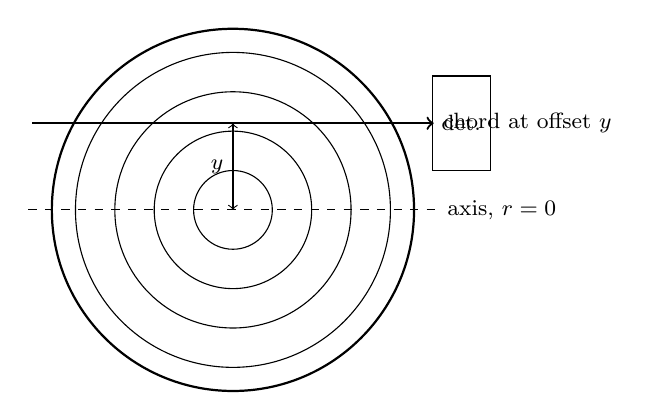
\begin{tikzpicture}[scale=1.0, every node/.style={font=\footnotesize}]
 \foreach \r in {0.5,1.0,1.5,2.0} {
 \draw[black,thin] (0,0) circle (\r);
 }
 \draw[black,thick] (0,0) circle (2.3);
 \draw[black,dashed] (-2.6,0) -- (2.6,0) node[right] {axis, $r=0$};
 \draw[black,thick,->] (-2.55,1.1) -- (2.55,1.1);
 \draw[black] (2.55,1.1) node[right] {chord at offset $y$};
 \draw[black,<->] (0,0) -- (0,1.1) node[midway,left] {$y$};
 \draw[black] (2.9,1.1) node[draw,rectangle,minimum width=0.4cm,minimum height=1.2cm] {det.};
\end{tikzpicture}
\caption{Schematic (illustrative, not measured) geometry for line-of-sight integration through a cylindrically symmetric emitting plasma column. A chord at perpendicular offset $y$ records the integral of Eq.~\eqref{eq:oes-los}; a set of such chords at different $y$ is required as input to the Abel inversion of Eq.~\eqref{eq:oes-abelinv}.}
\label{fig:oes-abel-schematic}
\end{figure}

\subsection{Representative diagnostic transitions}

Table~\ref{tab:oes-lines} lists, for orientation, representative upper-level energies and decay rates for transitions commonly exploited in argon and helium line-ratio and CR-model diagnostics. The values are illustrative, order-of-magnitude figures typical of the $4p\to4s$ argon manifold and the singlet/triplet helium system used throughout this chapter's cited works; they are not measurements from this work, nor a substitute for a validated atomic database.

\begin{table}[htbp]
\centering
\caption{Illustrative order-of-magnitude atomic parameters for representative visible transitions used in OES electron-temperature diagnostics. Values are indicative only, not experimental data from this work.}
\label{tab:oes-lines}
\begin{tabular}{@{}llcc@{}}
\toprule
Species & Transition class & Upper-level energy $E_{p}$ (\si{\eV}) & Decay rate $A_{p}$ (\si{\per\second}) \\
\midrule
Ar\,\textsc{i} & $4p\to4s$ manifold & $\sim 13$--$15$ & $\sim 10^{7}$--$10^{8}$ \\
He\,\textsc{i} & singlet ($3^{1}D\to2^{1}P$) & $\sim 23$ & $\sim 10^{7}$ \\
He\,\textsc{i} & triplet ($3^{3}D\to2^{3}P$) & $\sim 23$ & $\sim 10^{7}$ \\
Xe\,\textsc{i} & $6p\to6s$ manifold & $\sim 9$--$11$ & $\sim 10^{6}$--$10^{7}$ \\
\bottomrule
\end{tabular}
\end{table}

Figure~\ref{fig:oes-rate-curve} illustrates the strongly nonlinear sensitivity of a threshold-type excitation rate coefficient to $T_{\mathrm{e}}$ underlying the line-ratio sensitivity of Section~\ref{sec:oes-lineratio}, using the Arrhenius-type model of Eq.~\eqref{eq:oes-arrhenius} for two threshold energies.

\begin{figure}[htbp]
\centering
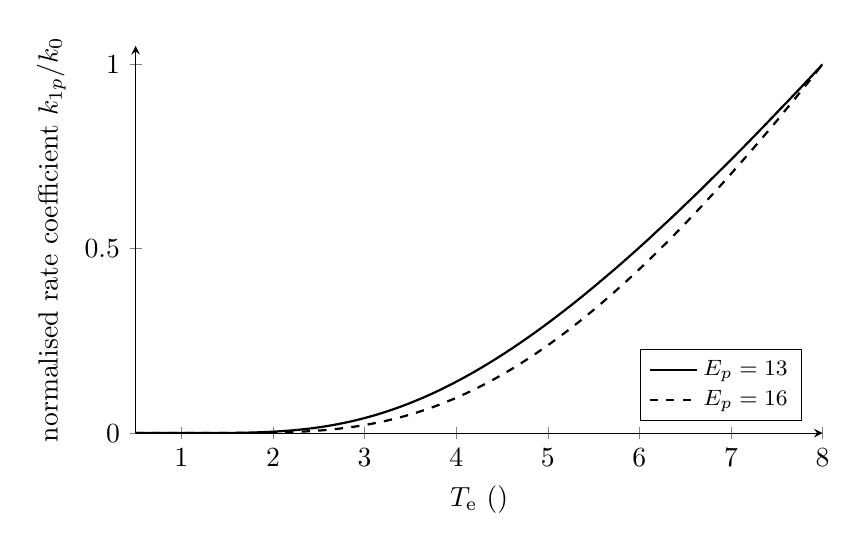
\begin{tikzpicture}
\begin{axis}[
 width=0.85\linewidth, height=6.5cm,
 xlabel={$T_{\mathrm{e}}$ (\si{\eV})},
 ylabel={normalised rate coefficient $k_{1p}/k_{0}$},
 domain=0.5:8, samples=120,
 xmin=0.5, xmax=8, ymin=0, ymax=1.05,
 axis lines=left,
 legend pos=south east,
 legend style={font=\footnotesize},
 every axis plot/.append style={thick, black},
]
\addplot[black, solid] {sqrt(x/8)*exp(-13/x)/ (sqrt(1)*exp(-13/8))};
\addlegendentry{$E_{p}=\SI{13}{\eV}$}
\addplot[black, dashed] {sqrt(x/8)*exp(-16/x)/ (sqrt(1)*exp(-16/8))};
\addlegendentry{$E_{p}=\SI{16}{\eV}$}
\end{axis}
\end{tikzpicture}
\caption{Schematic, analytic illustration (not measured data) of the strongly nonlinear dependence of a threshold-type Maxwellian-averaged excitation rate coefficient, Eq.~\eqref{eq:oes-arrhenius}, on $T_{\mathrm{e}}$, normalised to its value at $T_{\mathrm{e}}=\SI{8}{\eV}$, for two threshold energies $E_{p}$. The differential sensitivity between the curves is the physical basis of two-line electron-temperature thermometry.}
\label{fig:oes-rate-curve}
\end{figure}

\section{Strengths and Limitations}

\subsection{Strengths}

The passivity of OES translates into concrete practical advantages over material-probe diagnostics. Because no surface is inserted, there is no local perturbation of the sheath, the presheath field, or the ambient particle and energy fluxes — valuable when the goal, as here, is to characterise the very boundary layer a probe would otherwise disturb. There is no probe contamination or sputtering, no biasing or arcing risk in electronegative or high-density plasmas, and no restriction to plasmas accessible to a mechanically inserted tip, so OES functions equally well in high-density, high-power, or hazardous discharges (magnetron sources, Hall thrusters, atmospheric-pressure jets) where a Langmuir probe would be destroyed, draw prohibitive current, or be geometrically inaccessible. It is also remote and non-contact, compatible with real-time process monitoring and with energetic environments such as thruster exhaust plumes \cite{ref0256,ref0257} where material probes erode severely. Finally, because the same spectrum can, in favourable cases, simultaneously yield $T_{\mathrm{e}}$, $n_{\mathrm{e}}$, relative species densities (actinometry), gas temperature (molecular bands), and, via Doppler broadening, heavy-particle temperature, OES offers a rich, multi-parameter return on one minimally invasive measurement.

\subsection{Limitations}

These strengths are counterbalanced by real limitations. First, OES measures only what the plasma radiates and provides no direct measurement of the ion velocity distribution $f_{\mathrm{i}}(v)$, the ion flux, or the sheath potential profile — the central quantities of this monograph — which must come from complementary techniques combined with OES-derived $T_{\mathrm{e}}$ and $n_{\mathrm{e}}$. Second, accuracy is only as good as the CR model and cross-section database used in the inversion of Eq.~\eqref{eq:oes-chisq}; disagreements of tens of per cent against the Langmuir probe are not uncommon, traceable to incomplete cascade or metastable treatment, missing non-Maxwellian corrections, or outdated cross-section data — cross-comparison against an electrostatic-probe benchmark has repeatedly been used to quantify this \cite{ref0266}. Third, a chordal measurement without Abel inversion or tomography returns only an emissivity-weighted average, obscuring gradients expected across a thin presheath unless spatial resolution is engineered by narrow optics, translation scanning, or tomography. Fourth, the coronal-limit formulas that make OES tractable break down as $n_{\mathrm{e}}$ rises toward the regime where stepwise excitation and quenching become significant. Finally, actinometry assumes the admixed gas does not itself perturb the plasma chemistry at the concentration needed for adequate signal — an assumption that must be checked, not asserted, in reactive discharges.

\section{Role in the Multi-Diagnostic Fusion}

No single diagnostic treated here — Langmuir probe, laser-induced fluorescence, retarding-field energy analyser, or OES — is individually sufficient to constrain the full set of quantities entering the ion energy flux delivered across the plasma sheath,
\begin{equation}
\Gamma_{E} = \int q\,\phi_{\mathrm{tot}}(v)\, v\, f_{\mathrm{i}}(v)\, \mathrm{d}v ,
\label{eq:oes-gammae}
\end{equation}
where $\phi_{\mathrm{tot}}$ is the total energy (kinetic plus sheath acceleration) acquired by an ion of speed $v$ crossing the sheath, and $f_{\mathrm{i}}(v)$ is the ion velocity distribution at the sheath edge. Evaluating Eq.~\eqref{eq:oes-gammae}, or its Bohm-flux approximation $\Gamma_{E}\approx n_{\mathrm{e}} u_{\mathrm{B}} \langle E_{\mathrm{i}}\rangle$ with $u_{\mathrm{B}}=\sqrt{T_{\mathrm{e}}/M_{\mathrm{i}}}$ the Bohm velocity, requires $n_{\mathrm{e}}$ and $T_{\mathrm{e}}$ at the sheath edge, the sheath potential drop setting mean ion impact energy, and, for a fully kinetic treatment, the shape of $f_{\mathrm{i}}(v)$ itself. Within this book's diagnostic strategy, OES supplies the bulk-plasma or presheath-edge $n_{\mathrm{e}}$ and $T_{\mathrm{e}}$ that anchor the Bohm-velocity prefactor and, through the Debye length $\lambda_{\mathrm{D}} = \sqrt{\varepsilon_{0}T_{\mathrm{e}}/(n_{\mathrm{e}}e^{2})}$, the sheath thickness scale used throughout earlier chapters — supplied non-invasively, without the geometric and current-collection uncertainties of Langmuir-probe analysis. Laser-induced fluorescence and Doppler-resolved OES line widths independently constrain the ion temperature $T_{\mathrm{i}}$ and the ion velocity distribution's shape, cross-checking the Boltzmann or Maxwellian assumptions used to interpret OES line ratios. The retarding-field energy analyser and Langmuir probe supply direct in-situ measurements of the ion energy distribution and local floating and plasma potentials that OES cannot access, but at the cost of a physically inserted, current-collecting surface whose perturbation of the local sheath structure is exactly the quantity being measured. This cross-referencing is not merely a convenience: because each diagnostic is sensitive to a different moment or spatial region of the plasma, systematic comparison — OES against an electrostatic-probe benchmark \cite{ref0266} — is the principal available check on the accuracy of any single method, and standard practice wherever OES is deployed among several diagnostics characterising electric-propulsion discharges \cite{ref0256,ref0257} or industrial processing plasmas. The division of labour adopted here: OES furnishes the passively measured $n_{\mathrm{e}}(x)$ and $T_{\mathrm{e}}(x)$ profile feeding the Bohm-criterion boundary condition; Langmuir-probe and retarding-field-analyser data furnish the local potential structure and directly sampled ion energy distribution; and laser-induced-fluorescence Doppler measurements furnish an independent ion velocity distribution against which fluid-model closure assumptions can be tested. No measurement in this triad is redundant: each closes a different gap in the chain of inference to $\Gamma_{E}$ of Eq.~\eqref{eq:oes-gammae}, and only the combination yields an ion energy flux estimate whose uncertainty budget is fully closed.

\subsection{Summary}

Optical emission spectroscopy extracts $T_{\mathrm{e}}$ and $n_{\mathrm{e}}$ from the plasma's own light, exploiting the threshold-governed sensitivity of electron-impact excitation rate coefficients through two-line-ratio and actinometric methods, and, more rigorously, through inversion of a full collisional-radiative population balance spanning the coronal and LTE limits as special cases. Reliable quantitative use demands a validated cross-section database; careful wavelength and, where absolute intensities are required, radiometric calibration; explicit treatment of line-of-sight integration, via Abel inversion or tomography, whenever spatial resolution across a gradient region such as a presheath is required; and an honest accounting of errors from cascading, metastable pumping, self-absorption, and non-Maxwellian populations. Set against these demands are the technique's decisive practical virtues — passive, non-perturbing, remote, and compatible with plasma regimes inaccessible to material probes — which is why OES occupies a permanent place alongside the Langmuir probe, the retarding-field energy analyser, and laser-induced fluorescence in the multi-diagnostic strategy used here to constrain the electron-side boundary conditions, the Debye and sheath length scales, and, ultimately, the ion energy flux $\Gamma_{E}$ across the plasma sheath.
